% Options for packages loaded elsewhere
\PassOptionsToPackage{unicode}{hyperref}
\PassOptionsToPackage{hyphens}{url}
%
\documentclass[
  10pt,
]{article}
\usepackage{amsmath,amssymb}
\usepackage{iftex}
\ifPDFTeX
  \usepackage[T1]{fontenc}
  \usepackage[utf8]{inputenc}
  \usepackage{textcomp} % provide euro and other symbols
\else % if luatex or xetex
  \usepackage{unicode-math} % this also loads fontspec
  \defaultfontfeatures{Scale=MatchLowercase}
  \defaultfontfeatures[\rmfamily]{Ligatures=TeX,Scale=1}
\fi
\usepackage{lmodern}
\ifPDFTeX\else
  % xetex/luatex font selection
\fi
% Use upquote if available, for straight quotes in verbatim environments
\IfFileExists{upquote.sty}{\usepackage{upquote}}{}
\IfFileExists{microtype.sty}{% use microtype if available
  \usepackage[]{microtype}
  \UseMicrotypeSet[protrusion]{basicmath} % disable protrusion for tt fonts
}{}
\makeatletter
\@ifundefined{KOMAClassName}{% if non-KOMA class
  \IfFileExists{parskip.sty}{%
    \usepackage{parskip}
  }{% else
    \setlength{\parindent}{0pt}
    \setlength{\parskip}{6pt plus 2pt minus 1pt}}
}{% if KOMA class
  \KOMAoptions{parskip=half}}
\makeatother
\usepackage{xcolor}
\usepackage[margin=22mm]{geometry}
\usepackage{longtable,booktabs,array}
\usepackage{calc} % for calculating minipage widths
% Correct order of tables after \paragraph or \subparagraph
\usepackage{etoolbox}
\makeatletter
\patchcmd\longtable{\par}{\if@noskipsec\mbox{}\fi\par}{}{}
\makeatother
% Allow footnotes in longtable head/foot
\IfFileExists{footnotehyper.sty}{\usepackage{footnotehyper}}{\usepackage{footnote}}
\makesavenoteenv{longtable}
\usepackage{graphicx}
\makeatletter
\def\maxwidth{\ifdim\Gin@nat@width>\linewidth\linewidth\else\Gin@nat@width\fi}
\def\maxheight{\ifdim\Gin@nat@height>\textheight\textheight\else\Gin@nat@height\fi}
\makeatother
% Scale images if necessary, so that they will not overflow the page
% margins by default, and it is still possible to overwrite the defaults
% using explicit options in \includegraphics[width, height, ...]{}
\setkeys{Gin}{width=\maxwidth,height=\maxheight,keepaspectratio}
% Set default figure placement to htbp
\makeatletter
\def\fps@figure{htbp}
\makeatother
\setlength{\emergencystretch}{3em} % prevent overfull lines
\providecommand{\tightlist}{%
  \setlength{\itemsep}{0pt}\setlength{\parskip}{0pt}}
\setcounter{secnumdepth}{5}
\ifLuaTeX
  \usepackage{selnolig}  % disable illegal ligatures
\fi
\usepackage{bookmark}
\IfFileExists{xurl.sty}{\usepackage{xurl}}{} % add URL line breaks if available
\urlstyle{same}
\hypersetup{
  pdftitle={Cosmological Vacuum Selection and the Maximal Chronometric-Shear Ridge},
  pdfauthor={Technical research note v0.8},
  hidelinks,
  pdfcreator={LaTeX via pandoc}}

\title{Cosmological Vacuum Selection and the Maximal Chronometric-Shear
Ridge}
\usepackage{etoolbox}
\makeatletter
\providecommand{\subtitle}[1]{% add subtitle to \maketitle
  \apptocmd{\@title}{\par {\large #1 \par}}{}{}
}
\makeatother
\subtitle{Reheating, replicated-sector asymmetry, the QCD crossover,
matter locking, and parameter optimization in Z6 QCD chronometry}
\author{Technical research note v0.8}
\date{17 August 2026}

\begin{document}
\maketitle

{
\setcounter{tocdepth}{3}
\tableofcontents
}
\section{Executive result}\label{executive-result}

The cosmological calculation changes the preferred parameter region, but
does not kill the model.

The old local-screening benchmark,

\[
N=6,\qquad M=10\ {\rm TeV},\qquad f_a=M_{\rm Pl},\qquad \epsilon=10^{-6},
\]

has negligible thermal response:

\[
\eta_{\Psi,\max}=2.27\times10^{-7},\qquad
\eta_{\rm QCD,\max}=2.81\times10^{-7}.
\]

The early Universe therefore cannot select its vacuum. With a generic
displacement of order \(\pi/6\), its constant-mass misalignment estimate
is

\[
\Omega_a h^2\simeq 1.6\times10^2.
\]

That benchmark remains useful for local Earth-Sun screening, but it is
not a satisfactory generic cosmological benchmark.

A viable cosmological region instead lies on a lower-\(f_a\),
smaller-\(\epsilon\) ridge. The strongest fully evolved benchmark found
here is

\[
\boxed{
N=6,\quad
f_a=2.435\times10^{10}\ {\rm GeV},\quad
\epsilon=2.70\times10^{-13},\quad
M=1.002\times10^6\ {\rm GeV}
}
\]

with

\[
T_R=100M=1.002\times10^8\ {\rm GeV},\qquad
m_a=7.5\times10^{-29}\ {\rm eV},\qquad
d_g=10^{-6}.
\]

One adjacent replica is populated at reheating with temperature ratio

\[
\xi\equiv T_5/T_0=0.25.
\]

This gives

\[
\Delta N_{\rm eff}\simeq0.0289,
\]

below the current 95\% upper limit \(\Delta N_{\rm eff}<0.107\). The
heavy threshold and QCD crossover both dominate Hubble friction,

\[
\eta_{\Psi,\max}=612,
\qquad
\eta_{\rm QCD,\max}=759,
\]

and all 12 evenly spaced homogeneous initial phases tested numerically
converge to the same adjacent vacuum,

\[
\boxed{x_v=\frac{\pi}{6}},\qquad x\equiv a/f_a.
\]

The misalignment abundance is negligible,

\[
\Omega_a h^2\simeq2.3\times10^{-18}.
\]

The maximum generic chronometric signal is not set by cosmology. It
remains limited by equivalence-principle constraints. Taking the
conservative working value \(d_g=10^{-6}\), the predicted solar annual
peak-to-peak clock modulation is

\[
\boxed{
\left|\Delta\ln\frac{\nu_A}{\nu_B}\right|_{\rm yr}
\simeq 6.58\times10^{-22}\,|K_{AB}|.
}
\]

For an ordinary atomic sensitivity \(|K_{AB}|\sim1\), this is remote.
For the provisional nuclear sensitivity \(|K|\sim10^4\) used in recent
thorium-229 analyses, it becomes \(6.6\times10^{-18}\), although the
nuclear matrix-element uncertainty is substantial.

The main conceptual result is:

\[
\boxed{
\text{cosmology can select the sign and branch of chronometric shear,}
\text{ but it does not raise its allowed magnitude above the EP bound.}
}
\]

\section{Model}\label{model}

\subsection{Zero-temperature protected
potential}\label{zero-temperature-protected-potential}

The compact ratio mode is

\[
x=\frac{a}{f_a}.
\]

The replicated vectorlike thresholds are

\[
M_k(x)=M\left[1-\epsilon\cos\left(x+\frac{2\pi k}{N}\right)\right],
\qquad k=0,\ldots,N-1.
\]

The cyclic orbit cancels all lower harmonics in the vacuum effective
potential. For \(N>4\),

\[
V_0(x)=\frac{m_a^2f_a^2}{N^2}\left(1+\cos Nx\right),
\]

where

\[
m_a^2=
\frac{N_cN^2F_N}{8\pi^2}
\frac{M^4}{f_a^2}\epsilon^N,
\]

and

\[
F_N=
\frac{24\,2^{1-N}}
{(N-1)(N-2)(N-3)(N-4)}.
\]

The minima are

\[
x_v=\frac{(2j+1)\pi}{N}.
\]

The visible QCD threshold transmits the ratio-mode response as

\[
\mathrm d\ln\frac{\Lambda_3}{\chi}
=
\left[\frac{2}{27}+O(\alpha_s)\right]
\mathrm d\ln\frac{M_0}{\chi}.
\]

At a selected vacuum,

\[
d_g=
\frac{2}{27}\frac{M_{\rm Pl}}{f_a}
\frac{\epsilon\sin x_v}{1-\epsilon\cos x_v}.
\]

\subsection{Cosmological equation}\label{cosmological-equation}

The homogeneous field obeys

\[
\ddot x+3H\dot x+\frac{1}{f_a^2}\frac{\partial V_{\rm eff}}{\partial x}=0,
\]

with

\[
V_{\rm eff}=V_0+V_{\Psi,T}+V_{{\rm QCD},T}+V_b.
\]

The numerical evolution includes visible and hidden radiation, standard
matter, and a cosmological constant in \(H\).

\section{Reheating and the heavy-threshold thermal
potential}\label{reheating-and-the-heavy-threshold-thermal-potential}

For a Dirac colour triplet with \(g_\Psi=12\), the exact one-loop
thermal free-energy contribution is

\[
V_{\Psi,k}(T_k,x)
=-\frac{g_\Psi T_k^4}{2\pi^2}
\int_0^\infty dq\,q^2
\ln\left[1+e^{-\sqrt{q^2+M_k^2(x)/T_k^2}}\right].
\]

At leading order in \(\epsilon\),

\[
V_{\Psi,T}^{(1)}
=-\sum_k A_\Psi(T_k)
\cos\left(x+\frac{2\pi k}{N}\right),
\]

where

\[
A_\Psi(T)=
\epsilon M\frac{\partial V_\Psi(T,M)}{\partial M}.
\]

For \(T\gg M\),

\[
A_\Psi(T)\longrightarrow
\frac{g_\Psi}{24}\epsilon M^2T^2.
\]

Each decoupled replica conserves entropy independently:

\[
T_k g_{*s}^{1/3}(T_k)
=\xi_k T_0 g_{*s}^{1/3}(T_0).
\]

At high temperature, define the thermal phasor

\[
W_2=\sum_k\xi_k^2e^{2\pi ik/N}.
\]

Then

\[
V_{\Psi,T}^{(1)}\propto-\operatorname{Re}\left(e^{ix}W_2\right),
\qquad
x_T=-\arg W_2.
\]

For the benchmark population,

\[
\xi_0=1,\qquad \xi_5=0.25,
\]

and all other replicas are empty. Therefore

\[
W_2=1+0.25^2e^{-i\pi/3},
\qquad
\boxed{x_T=0.0524383}.
\]

This is a useful economy: the branch-selecting phase scales as
\(\xi^2\), while the dark-radiation cost scales as \(\xi^4\).

For a complete hidden Standard Model copy with its standard internal
neutrino-photon entropy history,

\[
\Delta N_{\rm eff}\simeq7.403\,\xi^4.
\]

Thus \(\xi=0.25\) gives

\[
\Delta N_{\rm eff}=0.0289.
\]

Only one adjacent copy can be populated at this level: five copies at
\(\xi=0.25\) would give \(\Delta N_{\rm eff}\simeq0.145\), above the
current bound.

\section{QCD crossover}\label{qcd-crossover}

For QCD pressure written as

\[
p(T,\Lambda)=T^4P(T/\Lambda),
\]

the thermodynamic identity

\[
\frac{\partial F}{\partial\ln\Lambda}\bigg|_T
=\rho-3p\equiv\Theta(T)
\]

follows directly from dimensional analysis.

The threshold relation gives

\[
\Lambda_k(x)=\Lambda_0
\left[1-\epsilon\cos\left(x+\frac{2\pi k}{N}\right)\right]^{2/27}.
\]

The leading lock-defect contribution is therefore

\[
V_{{\rm QCD},k}(T_k,x)
=\frac{2}{27}\Theta(T_k)
\ln\left[1-\epsilon\cos\left(x+\frac{2\pi k}{N}\right)\right].
\]

The evolution uses the \(2+1+1\)-flavour lattice trace-anomaly fit

\[
\frac{\Theta(T)}{T^4}
=e^{-h_1/t-h_2/t^2}
\left[
 h_0+f_0
 \frac{\tanh(f_1t+f_2)+1}
 {1+g_1t+g_2t^2}
\right],
\qquad t=\frac{T}{0.2\ {\rm GeV}},
\]

with

\[
(h_0,h_1,h_2,f_0,f_1,f_2,g_1,g_2)
=(0.353,-1.04,0.534,1.75,6.80,-5.18,0.525,0.160).
\]

For the strong benchmark, the QCD focusing measure peaks at

\[
T\simeq0.179\ {\rm GeV},
\qquad
\eta_{\rm QCD}\equiv\frac{4m_{T,{\rm QCD}}^2}{H^2}=759.
\]

The hidden sector crosses its own QCD region at a different visible
temperature. This produces a time-dependent phasor rather than a single
fixed thermal minimum.

\section{Matter domination}\label{matter-domination}

Nonrelativistic visible baryons contribute

\[
V_b(x,a)=\rho_b(a)
\left(1-\epsilon\cos x\right)^{p_b},
\qquad p_b\simeq\frac{2}{27}.
\]

Near the even-\(N\) thermal maximum \(x=0\), this gives a positive
curvature

\[
m_b^2(a)=\frac{\rho_b(a)p_b\epsilon}{f_a^2}.
\]

The zero-temperature potential gives a tachyonic curvature \(-m_a^2\).
The homogeneous branch is released when

\[
m_b^2(a)=m_a^2.
\]

Thus

\[
1+z_{\rm inst}=
\left[
\frac{m_a^2f_a^2}
{\rho_{b0}p_b\epsilon}
\right]^{1/3}.
\]

For the moderate and strong benchmarks,

\[
z_{\rm inst}=1224,
\qquad
z_{\rm inst}=450,
\]

respectively. Baryons do not screen the scalar in finite bodies, as
shown in v0.7, but the homogeneous cosmic baryon background can delay
the roll and alter the selected branch.

\section{Vacuum selection}\label{vacuum-selection}

\begin{figure}
\centering
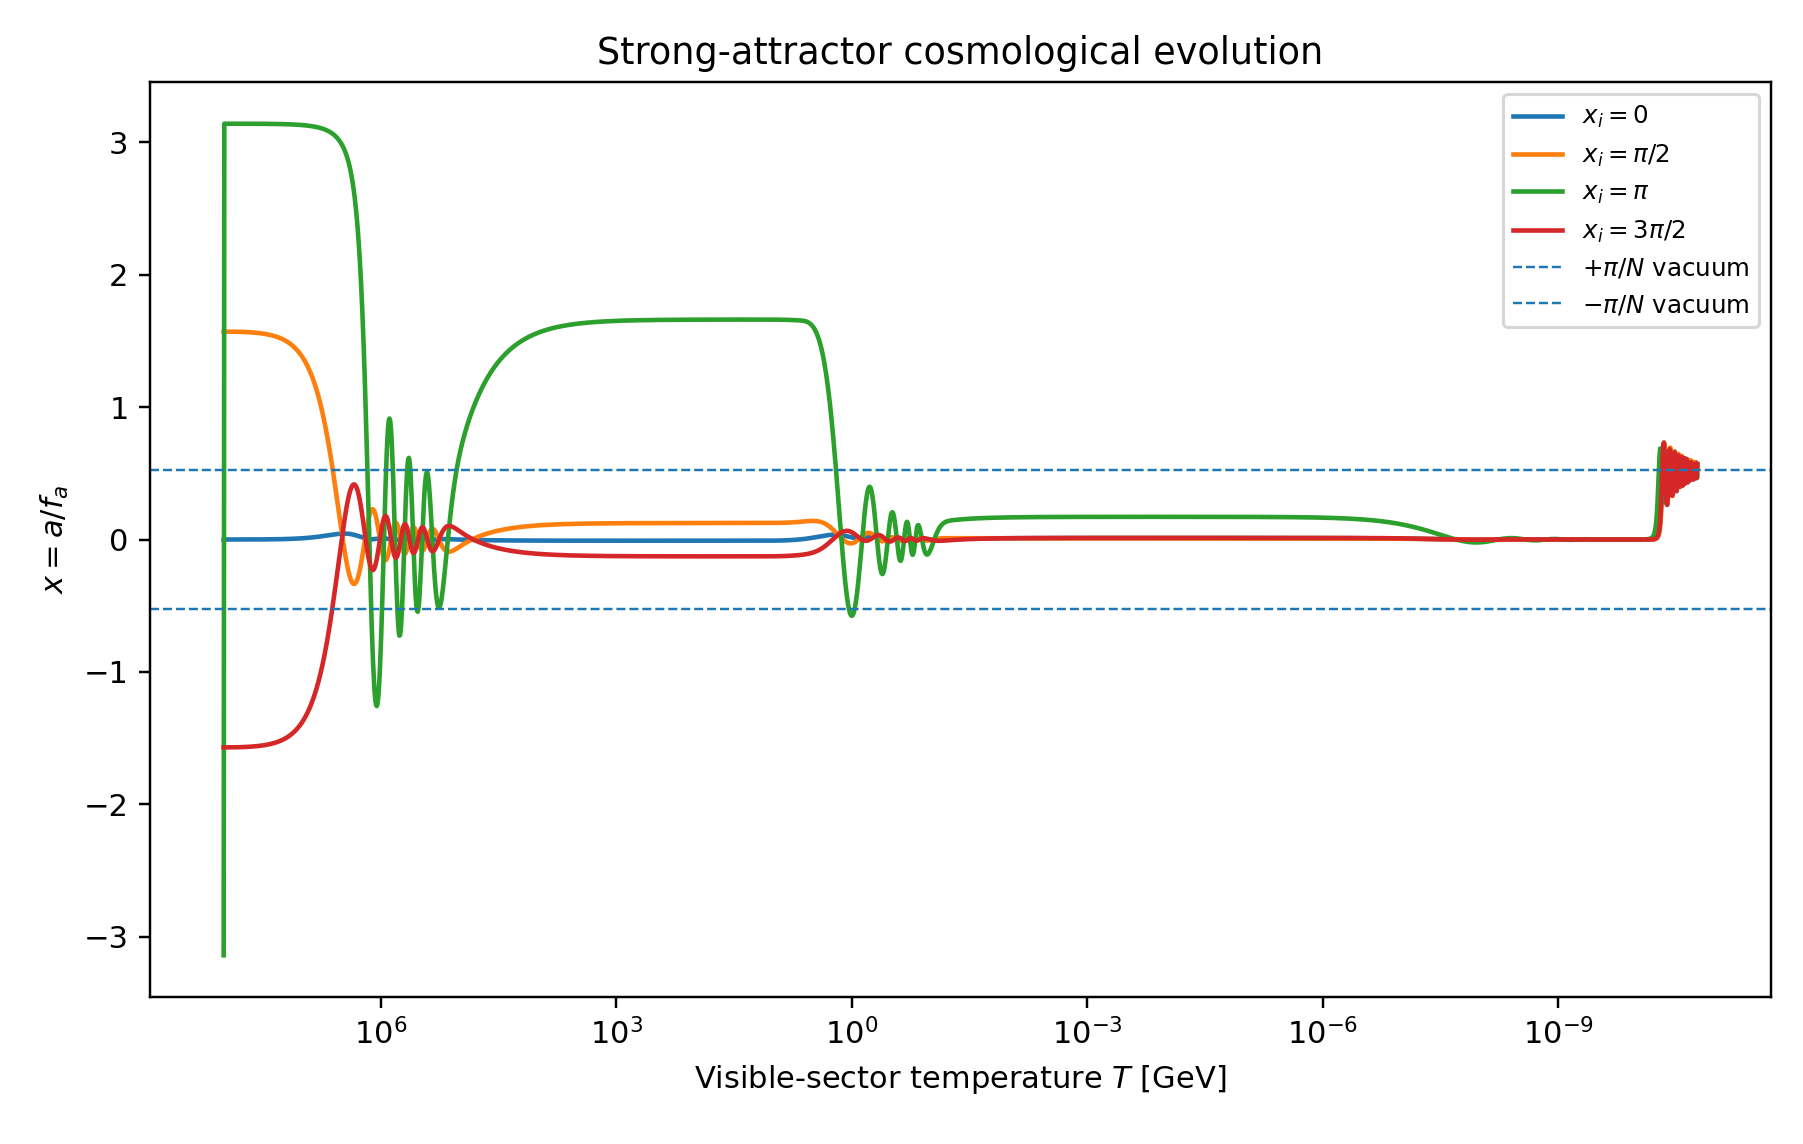
\includegraphics[width=0.95\textwidth,height=\textheight]{cosmological_vacuum_trajectory_v0_8.png}
\caption{Strong-attractor trajectories. Four widely separated
homogeneous initial phases converge to the same adjacent vacuum after
heavy-threshold focusing, QCD refocusing, baryon locking, and late
release.}
\end{figure}

\subsection{Moderate-focusing regime}\label{moderate-focusing-regime}

The moderate point is

\[
f_a=4.87\times10^{11}\ {\rm GeV},\quad
\epsilon=5.40\times10^{-12},\quad
M=5.01\times10^4\ {\rm GeV}.
\]

It has

\[
\eta_{\Psi,\max}=30.6,
\qquad
\eta_{\rm QCD,\max}=38.0.
\]

Nevertheless, a 12-point scan over the inflationary homogeneous phase
gives five trajectories in \(+\pi/6\) and seven in \(-\pi/6\). The
sudden disappearance of thermal curvature and subsequent QCD and
matter-era phase evolution preserve information about the initial zero
mode.

\subsection{Strong-attractor regime}\label{strong-attractor-regime}

The strong point is

\[
f_a=2.435\times10^{10}\ {\rm GeV},\quad
\epsilon=2.70\times10^{-13},\quad
M=1.002\times10^6\ {\rm GeV}.
\]

It has

\[
\eta_{\Psi,\max}=612,
\qquad
\eta_{\rm QCD,\max}=759.
\]

All 12 evenly spaced homogeneous initial phases tested converge to
\(+\pi/6\). The largest residual distance from that vacuum at the
numerical stopping surface is 0.049 rad.

\begin{figure}
\centering
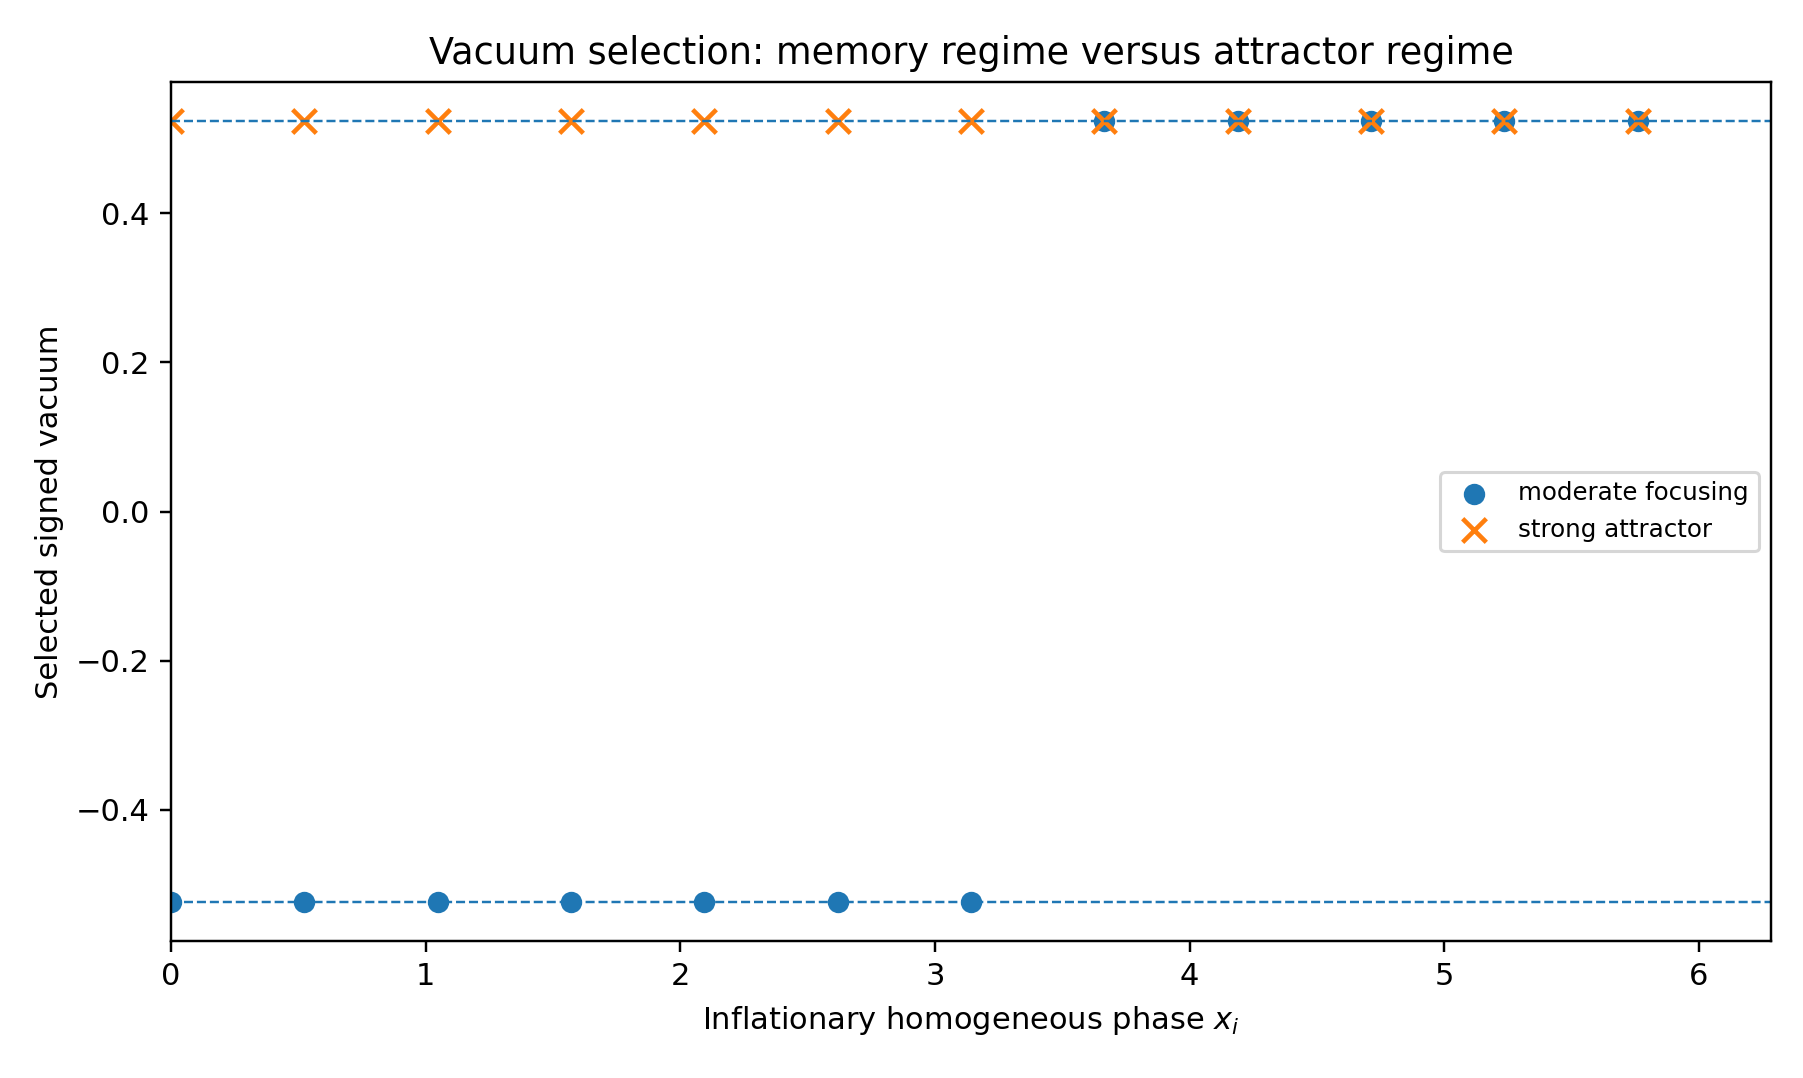
\includegraphics[width=0.95\textwidth,height=\textheight]{cosmological_vacuum_basin_v0_8.png}
\caption{The same reheating asymmetry produces a two-branch memory
regime at moderate focusing and a one-branch attractor in the tested
strong benchmark.}
\end{figure}

This is a numerical existence result, not a theorem that every point
with smaller \(f_a\) is a global attractor. Branch selection is
phase-sensitive and can form islands in parameter space.

\subsection{Domain-wall condition}\label{domain-wall-condition}

The exact zero-temperature theory retains \(Z_6\)-degenerate vacua. The
clean cosmology therefore requires:

\begin{enumerate}
\def\labelenumi{\arabic{enumi}.}
\tightlist
\item
  the approximate \(U(1)\) to break before or during inflation;
\item
  no post-inflation restoration, conservatively \(T_R<f_a\);
\item
  inflationary phase fluctuations smaller than the reheating bias.
\end{enumerate}

Since

\[
\delta x_{\rm inf}\simeq\frac{H_{\rm inf}}{2\pi f_a},
\]

a useful sufficient condition is

\[
H_{\rm inf}\ll2\pi f_a x_T.
\]

For the strong benchmark,

\[
2\pi f_ax_T=8.0\times10^9\ {\rm GeV}.
\]

If the symmetry is restored after inflation, an additional technically
safe permanent bias is required to remove strings and stable domain
walls. The transient reheating asymmetry alone is not a permanent
wall-lifting term.

\section{Why N=6 is preferred}\label{why-n6-is-preferred}

Visible-dominated reheating with even \(N\) focuses the field near a
zero-temperature maximum. The nearest minima are

\[
x_v=\pm\frac{\pi}{N}.
\]

For \(\epsilon\ll1\),

\[
d_g\simeq
\frac{2}{27}\frac{\epsilon}{y}
\sin\frac{\pi}{N},
\qquad y\equiv\frac{f_a}{M_{\rm Pl}}.
\]

At fixed \(d_g\),

\[
\epsilon=
\frac{27}{2}
\frac{d_g y}{\sin(\pi/N)}.
\]

The smallest even \(N>4\) is \(N=6\), which simultaneously gives:

\begin{itemize}
\tightlist
\item
  the largest adjacent-vacuum slope among allowed even \(N\);
\item
  the fewest replicated sectors;
\item
  the lowest heavy threshold required for a chosen \(m_a\);
\item
  the least severe reheating architecture.
\end{itemize}

For \(N=6\),

\[
\boxed{\epsilon=27d_gy}.
\]

The exact coloured-fermion thermal function gives

\[
\eta_{\Psi,\max}
\simeq0.22673\frac{\epsilon}{y^2}
=6.12\times10^{-6}
\left(\frac{d_g}{10^{-6}}\right)\frac1y.
\]

Thus thermal selection becomes stronger as \(f_a\) decreases, even
though \(\epsilon\) decreases.

\section{EP-saturating parameter
ridge}\label{ep-saturating-parameter-ridge}

The optimization uses the conservative working cap

\[
d_g=10^{-6},
\]

motivated by a leading pure-QCD recast of MICROSCOPE. It is not a
substitute for a complete likelihood including all dilaton charges and
finite-range effects.

The scan fixes

\[
m_a=7.5\times10^{-29}\ {\rm eV}
\]

as a representative late-roll mass and imposes

\[
T_R=100M<f_a,
\qquad
M>2.6\ {\rm TeV},
\qquad
M<10^{12}\ {\rm GeV},
\qquad
\eta_{\Psi,\max}>1.
\]

For \(N=6\), the mass relation reduces numerically to

\[
M\simeq
\frac{1.002\times10^{-2}\ {\rm GeV}}{y}
\left(\frac{m_a}{7.5\times10^{-29}\ {\rm eV}}\right)^{1/2}
\left(\frac{10^{-6}}{d_g}\right)^{3/2}.
\]

The viable scan interval is approximately

\[
6.4\times10^{-10}\lesssim y\lesssim3.9\times10^{-6},
\]

or

\[
1.6\times10^9\ {\rm GeV}\lesssim f_a\lesssim9.4\times10^{12}\ {\rm GeV},
\]

with

\[
2.6\times10^3\ {\rm GeV}\lesssim M\lesssim1.6\times10^7\ {\rm GeV}.
\]

The \(N=8\) scan survives only at much higher threshold masses,

\[
4.2\times10^{-7}\lesssim y\lesssim7.5\times10^{-6},
\]

\[
1.1\times10^8\ {\rm GeV}\lesssim M\lesssim8.2\times10^9\ {\rm GeV}.
\]

No \(N=10\) point survives the same \(M<10^{12}\) GeV, reheating,
collider, and focusing cuts.

\begin{figure}
\centering
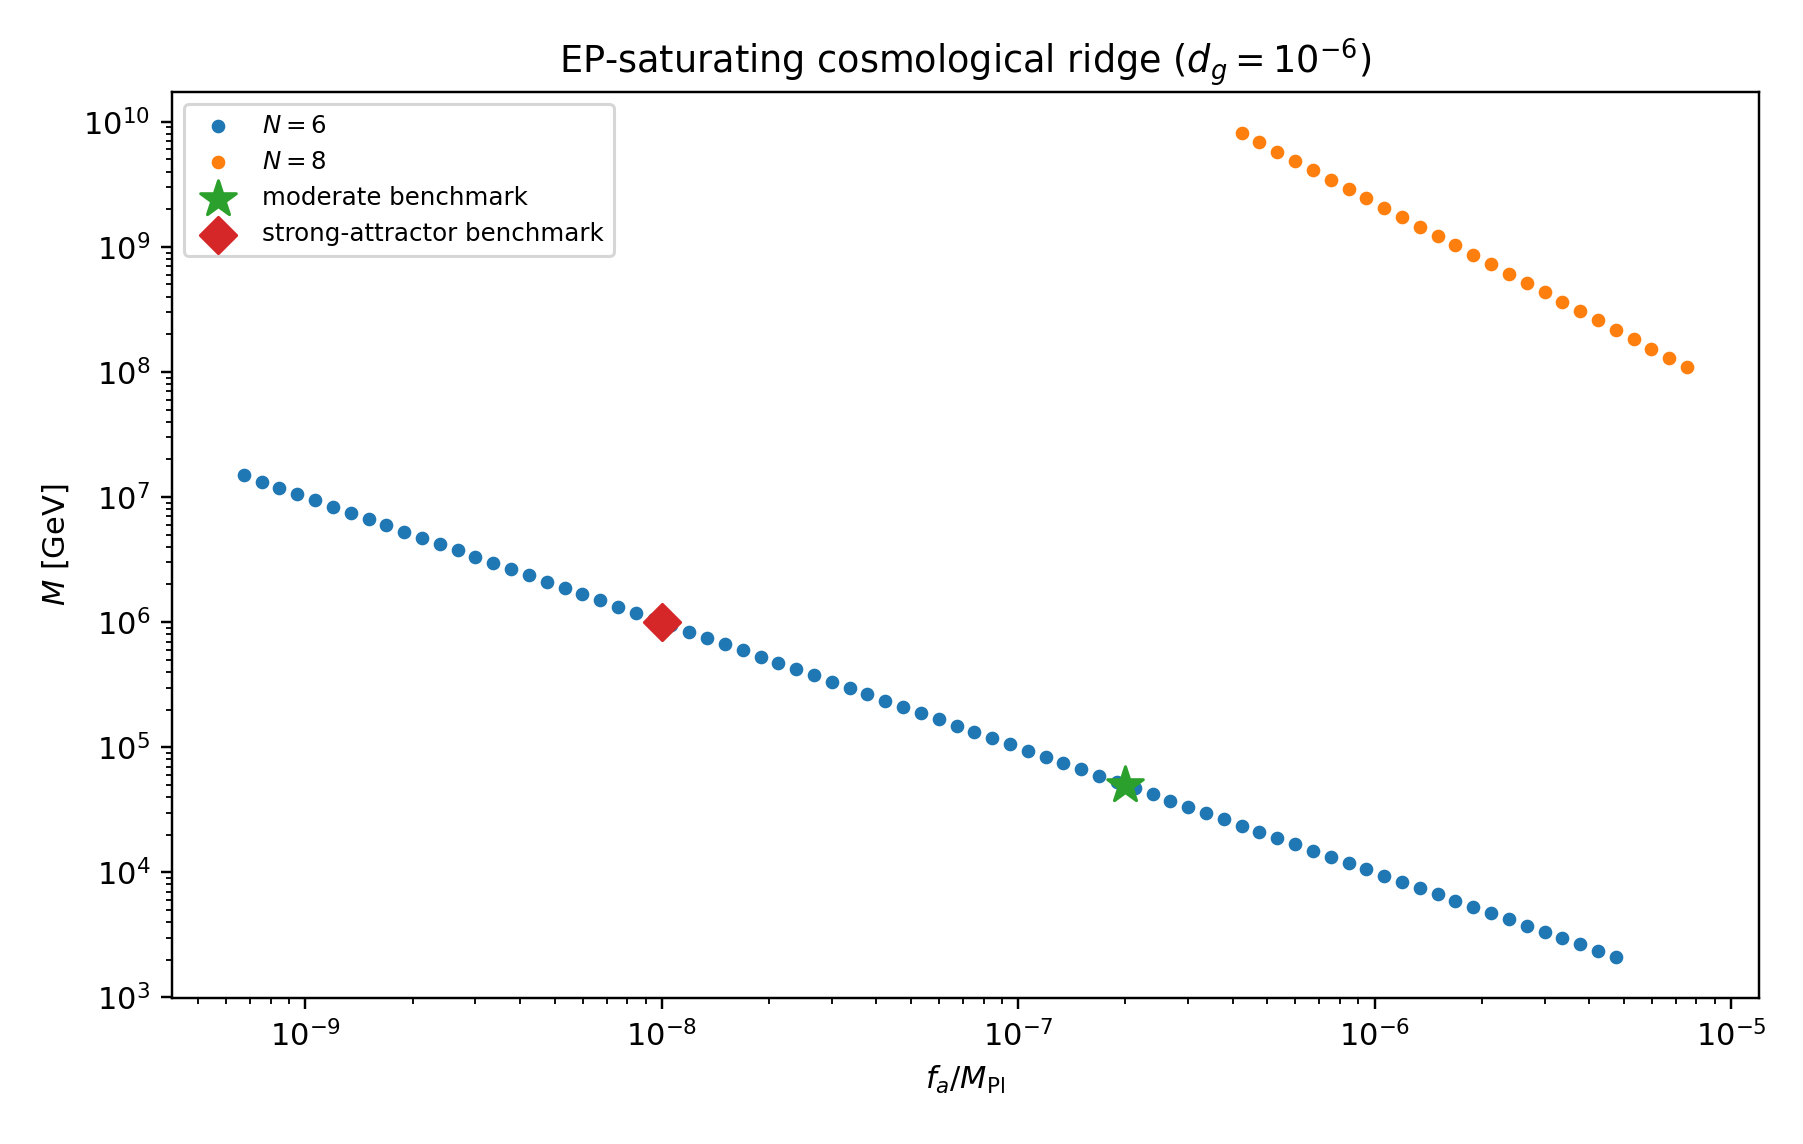
\includegraphics[width=0.95\textwidth,height=\textheight]{cosmological_parameter_ridge_v0_8.png}
\caption{The largest shear is a ridge rather than a unique point. N=6 is
parametrically and cosmologically cheaper than N=8.}
\end{figure}

\section{Force hierarchy and
chronology}\label{force-hierarchy-and-chronology}

\begin{figure}
\centering
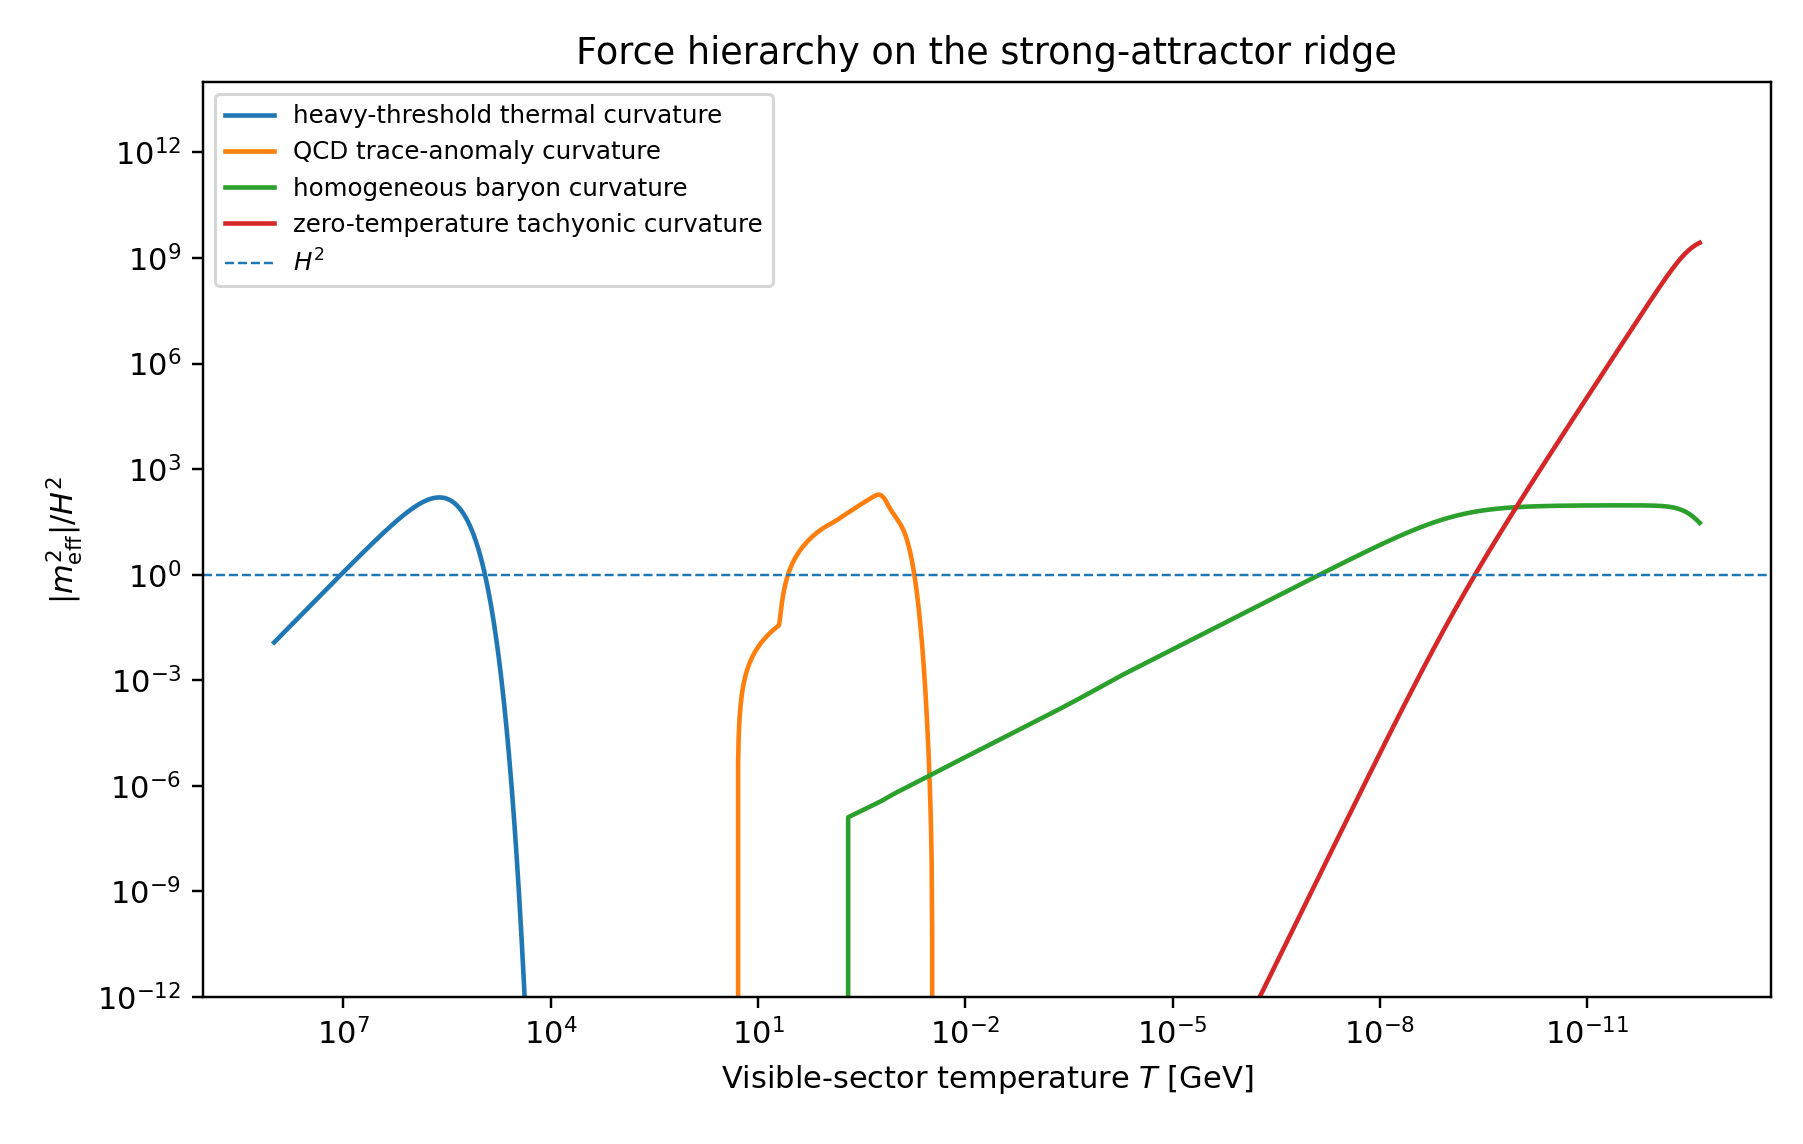
\includegraphics[width=0.95\textwidth,height=\textheight]{cosmological_force_hierarchy_v0_8.png}
\caption{The heavy threshold first focuses the phase, the QCD trace
anomaly refocuses it near 180 MeV, baryons hold it close to the even-N
maximum, and the zero-temperature tachyon finally releases it.}
\end{figure}

The sequence is:

\[
\boxed{
\text{reheating}
\rightarrow
\text{heavy-threshold focusing}
\rightarrow
\text{QCD refocusing}
\rightarrow
\text{baryon locking}
\rightarrow
\text{late tachyonic release}
\rightarrow
x_v=\pm\pi/6.
}
\]

The QCD crossover is dynamically important even though the final linear
coupling is generated by the zero-temperature threshold. It acts as a
second environmental lens for the same ratio mode.

\section{Chronometric shear}\label{chronometric-shear}

For two clocks,

\[
\mathcal S_{AB}=\mathrm d\ln\frac{\nu_A}{\nu_B}.
\]

In the pure-QCD benchmark,

\[
\mathcal S_{AB}
\simeq K_{AB}\,d_g\,\mathrm d\varphi,
\]

where \(K_{AB}\) is the difference in QCD/nuclear sensitivity and
\(\varphi=a/M_{\rm Pl}\).

A source with scalar charge approximately \(d_g\) produces

\[
\frac{a_{\rm source}}{M_{\rm Pl}}
\simeq-2d_g\Phi_N.
\]

For the annual peak-to-peak change of the solar potential,

\[
\Delta\Phi_\odot=3.29\times10^{-10},
\]

and \(m_a\ll {\rm AU}^{-1}\),

\[
\boxed{
\left|\Delta\ln\frac{\nu_A}{\nu_B}\right|_{\rm yr}
=2|K_{AB}|d_g^2\Delta\Phi_\odot.
}
\]

At \(d_g=10^{-6}\),

\[
\left|\Delta\ln\frac{\nu_A}{\nu_B}\right|_{\rm yr}
=6.58\times10^{-22}|K_{AB}|.
\]

Recent thorium-229 work uses provisional strong-sector sensitivity
factors \(|K_g|,|K_{\hat m}|=10^4\) and \(10^5\), while emphasizing that
reliable ab-initio coefficients are not yet available. Taking \(10^4\)
only as an illustrative benchmark gives

\[
6.58\times10^{-18}.
\]

This is a source-induced annual signal, not an oscillating-dark-matter
signal: the scalar abundance on the optimized ridge is negligible.

The clock/EP consistency relation derived in v0.5 remains

\[
\frac{\beta_{AB}}{\eta_{CD}}
=-\frac{\Delta K_{AB}}
{\Delta Q_{\hat m}^{\prime\,CD}},
\]

under the one-scalar, unscreened, QCD-dominated assumptions.
Cosmological vacuum selection fixes the sign of \(d_g\), but the ratio
above is independent of its magnitude.

\section{Abundance and cosmological
consistency}\label{abundance-and-cosmological-consistency}

For a constant mass that begins oscillating in radiation domination,

\[
\Omega_a h^2\propto f_a^2m_a^{1/2}\theta_i^2.
\]

The old Planck-scale benchmark gives \(\Omega_a h^2\simeq164\) for
\(\theta_i=\pi/6\). The moderate and strong ridge points give

\[
9.2\times10^{-16},
\qquad
2.3\times10^{-18},
\]

respectively. The ratio mode is therefore not the dark matter in the
optimized chronometric model.

The strong benchmark also satisfies

\[
\frac{T_R}{f_a}=4.11\times10^{-3},
\]

which is compatible with avoiding radial-symmetry restoration for
order-one thermal couplings, although the actual restoration temperature
depends on the UV completion.

Outstanding cosmological requirements are:

\begin{itemize}
\tightlist
\item
  an explicit reheaton producing \(\xi_0=1\), \(\xi_5=0.25\), and
  negligible temperatures in the other replicas;
\item
  prompt decays or acceptable relic abundances for the heavy vectorlike
  thresholds;
\item
  a perturbation/isocurvature calculation rather than only homogeneous
  evolution;
\item
  proof that the chosen reheating hierarchy is stable under portals
  between replicas;
\item
  a permanent domain-wall cure if pre-inflation symmetry breaking is not
  imposed.
\end{itemize}

\section{Novelty boundary}\label{novelty-boundary}

The following ingredients are established:

\begin{itemize}
\tightlist
\item
  nonlinearly realized \(Z_N\) protection of a light pseudo-Goldstone
  potential;
\item
  replicated-sector finite-temperature scalar cosmology;
\item
  lattice QCD thermodynamics;
\item
  dilaton equivalence-principle charges;
\item
  clock searches for gluon and quark-mass couplings.
\end{itemize}

The candidate new package is narrower:

\[
\boxed{
\begin{gathered}
\text{protected real vectorlike-QCD threshold}
+\frac{2}{27}\text{ transmission}
+\text{entropy-asymmetric reheating phasor}
\\
+\text{lattice trace-anomaly evolution}
+\text{baryon locking}
+\text{chronometric shear/EP ridge}.
\end{gathered}
}
\]

The most important new negative result is also useful: moderate thermal
focusing does not guarantee unique vacuum selection. The system can
retain the inflationary homogeneous phase through threshold decoupling
and later environmental kicks. A strong-attractor island exists, but it
must be demonstrated rather than inferred from \(m_T/H>1\) alone.

\section{Current verdict}\label{current-verdict}

\begin{longtable}[]{@{}
  >{\raggedright\arraybackslash}p{(\columnwidth - 2\tabcolsep) * \real{0.5000}}
  >{\raggedright\arraybackslash}p{(\columnwidth - 2\tabcolsep) * \real{0.5000}}@{}}
\toprule\noalign{}
\begin{minipage}[b]{\linewidth}\raggedright
Target
\end{minipage} & \begin{minipage}[b]{\linewidth}\raggedright
Verdict
\end{minipage} \\
\midrule\noalign{}
\endhead
\bottomrule\noalign{}
\endlastfoot
Heavy-threshold thermal evolution & Pass \\
Independent replica entropy histories & Pass within decoupled-sector
approximation \\
QCD crossover & Pass at leading lock defect \\
Matter domination & Pass \\
Local Earth/Sun screening & Pass from v0.7: unscreened \\
Unique branch at moderate focusing & Fail \\
Unique branch at strong benchmark & Pass for 12 tested homogeneous
phases \\
Dark-radiation bound & Pass for one adjacent copy at \(\xi=0.25\) \\
Misalignment abundance & Pass; negligible \\
Maximum nonzero chronometric shear & EP-limited at working
\(d_g\sim10^{-6}\) \\
Permanent domain-wall solution & Conditional/open \\
Full reheating UV completion & Open \\
Absolute priority claim & Not yet established \\
\end{longtable}

The preferred cosmological statement is now:

\[
\boxed{
\text{N=6 admits a low-}f_a\text{ attractor ridge on which the Universe}
\text{ selects a nonzero QCD chronometric-shear vacuum.}
}
\]

It is not the origin of causal order. It is a concrete mechanism by
which cosmological history selects which small, non-universal spectral
mismatch survives after a universal clock scale has formed.

\section{References}\label{references}

\begin{enumerate}
\def\labelenumi{\arabic{enumi}.}
\tightlist
\item
  S. Das and A. Hook, \emph{Non-linearly realized discrete symmetries},
  arXiv:2006.10767.
\item
  D. Brzeminski, Z. Chacko, A. Dev and A. Hook, \emph{A Time-Varying
  Fine Structure Constant from Naturally Ultralight Dark Matter},
  arXiv:2012.02787.
\item
  S. Borsanyi et al., \emph{Lattice QCD for Cosmology},
  arXiv:1606.07494.
\item
  S. Goldstein and J. C. Hill, \emph{A 2\% determination of N\_eff from
  primordial element abundance, CMB and BAO measurements},
  arXiv:2603.13226.
\item
  P. Touboul et al., \emph{MICROSCOPE mission: final results of the test
  of the Equivalence Principle}, arXiv:2209.15487.
\item
  T. Damour and J. F. Donoghue, \emph{Equivalence Principle Violations
  and Couplings of a Light Dilaton}, arXiv:1007.2792.
\item
  J. Arakawa et al., \emph{Probing Ultralight Dark Matter at the
  Mega-Planck Scale with the Thorium Nuclear Clock}, arXiv:2602.16804.
\end{enumerate}

\end{document}
